\subsection{Motivi per fondare una startup}
Ci sono due (possibili) motivi principali per fondare una startup:
\begin{itemize}
 \item successo
 \item guadagno
\end{itemize}

Gli startupper che mirano alla fama cercano di rimanerne il più tempo possibile
``in sella'', rimandando l'exit (poiché in seguito la fama calerebbe). Per fare 
ciò è necessario diluirsi meno che si può nel tempo (ciò vendere meno quote 
possibile dell'azienda) ed essere più selettivi negli investitori che vengono 
scelti. Ciò determina anche un minor guadagno, in quanto lo startupper ha un 
reale ritorno al momento dell'exit.

All'inizio di un nuovo progetto è necessario decidere quale strategia adottare:
se massimizzare il risultato del progetto e l'aspetto economico o se
massimizzare la fama personale. In base a ciò vanno scelti determinati
investitori, che dovrebbero condividere la stessa visione, altrimenti si
potrebbero verificare situazioni conflittuali.

\subsection{Due tipi di investitori}

Esistono due tipi di investitori:
\begin{itemize}
 \item finanziario
 \item industriale
\end{itemize}

Gli investitori \textbf{finanziari} sono Business Angels o Venture Capital, i
quali puntano alla pura speculazione finanziaria: vogliono moltiplicare il
capitale investito. Mirano, quindi, all'aumento del valore delle quote per poi
rivenderle, indipendentemente da dal campo in cui lavora la startup. 

Gli investitori \textbf{industriali}, invece, sono investitori (principalmente
aziende) che, selezionando un numero ristretto di start-up, investono in
maniera più selettiva dove trovano un progetto che può essere ritenuto
interessante nella loro area di competenza.

Le differenze cruciali tra i due sono:
\begin{itemize}
 \item L'investitore industriale può fornire supporto tecnologico
 (partnership). Lo svantaggio è che in questa maniera l'investitore industriale
 potrebbe pretendere il controllo della \textit{governance} della startup oppure
 essere ingerente nei suoi confronti.
 \item L'investitore finanziario guarda agli aspetti finanziari della startup,
 ovvero solo al ritorno monetario. Viceversa, l'investitore industriale è più
 tollerante nelle fluttuazioni del successo che può avere l'operazione e non è
 interessato solamente ai risultati finanziari, ma anche ai risvolti
 tecnici/industriali (caso estremo: la startup non vende praticamente nulla ma
 risolve un problema tecnico di un altro prodotto dell'azienda).
 \item L'obiettivo finale dei due investitori è molto diverso. Il finanziario
 mira solamente all'exit finale. L'investitore industriale potrebbe non voler
 l'exit ma addirittura mirare al consolidamento interno del gruppo, ovvero
 ottenere la maggioranza delle quote e integrare la startup nel gruppo
 aziendale.
\end{itemize}

Un founder che sceglie un investitore industriale ha già trovato l'exit
finale.
Questa strada è ottima come scelta, ma preclude, solitamente, la possibilità di
avere investitori finanziari. Si ha quindi di fatto, una \textbf{scelta
esclusiva}. Ciò deriva dal fatto che gli investitori finanziari si potrebbero
ritrovare con dei capitali bloccati che non saranno in grado di recuperare con
un exit. Un founder deve prestare attenzione nel caso di soluzioni miste: si
rischia, infatti, che l'investitore finanziario si accordi
con quello industriale per farlo arrivare (almeno) al 51\% delle quote . In
questo caso, il fondatore stesso si  ritroverà ad avere il proprio capitale
bloccato. Infatti, ottenuta la maggioranza, gli investitori non avranno più
interesse a comprare le quote della startup.

La soluzione migliore è quindi di trovare un accordo di vendita con
l'investitore industriale, al quale cedere la maggior parte delle quote
(mantenendo solo, per esempio, il 5\% totale, più per orgoglio che per
effettiva rendita). In tal modo è possibile effettuare l'exit e capitalizzare
il più possibile.

Come si può valutare la propria startup? Non è semplice. Le vendite di
quota delle startup dovrebbero essere ampie all'inizio, per poi diminuire man
mano, alzando il prezzo. Un andamento contrario, chiamato \textit{down round},
può dare al mercato la percezione di un andamento negativo della startup.
Inoltre una vendita a prezzi minori delle nei successivi round potrebbe
indispettire gli investitori.

\subsection{Golden parachute (o paracadute d'oro)}
Una volta ottenuta la maggioranza da parte di un investitore, a meno di
clausole nel contratto di vendita delle quote, è discrezione di chi possiede la
maggioranza decidere se mantenere il corrente amministratore delegato o
cambiarlo. Per evitare questo tipo di situazioni è importante prevedere un
\textit{paracadute d'oro}, ovvero delle clausole in cui si pongono delle
condizioni di assunzione per un certo numero di anni (solitamente con uno
stipendi corposo) e, nel caso di una rimozione dall'incarico, una liquidazione
cospicua (che può prevedere anche il pagamento di tutti gli stipendi fino al
termine previsto dal contratto).

\chapter{Brand}

Come nella moda, anche nel mondo della tecnologia esistono i \textbf{trend}
(mode). Essi oscillano e si muovono nel tempo.

Quali sono le difficoltà lato startupper e lato sviluppatori? Si tratta di
capire le necessità del periodo per ottenere dei ritorni.

Come capire \textbf{quando è il momento di investire in un trend}?
Ci sono diverse modalità per capirlo.

La \textit{Gartner}, azienda multinazionale per l'analisi del mercato e
consulenza aziendale, presenta un approccio orientato alle tecnologie. Tra gli
strumenti che mette a disposizione è presente l'\textbf{hype cycle}.
Si osserva che tutte le tecnologie tendono a percorrere un andamento come
descritto in Figura~\ref{fig:hypecycle}.

\begin{figure}[H]
\centering
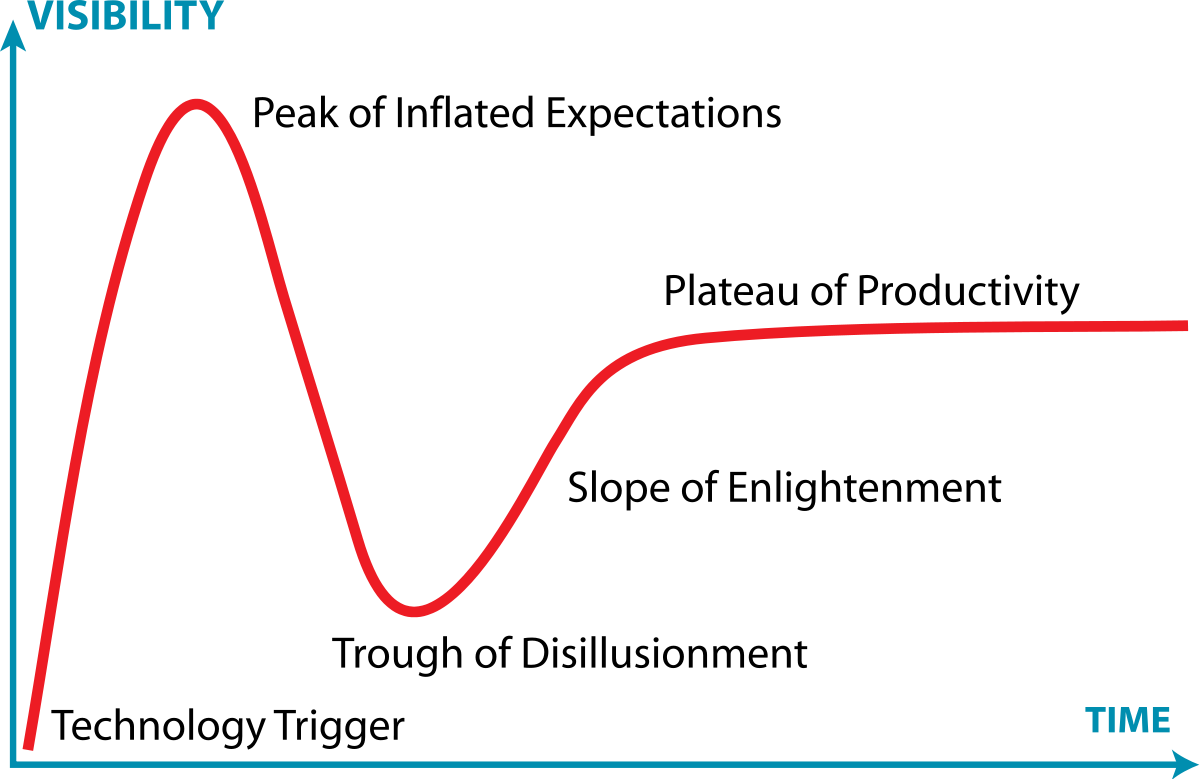
\includegraphics[scale=0.25]{hypecycle.png}
\caption[Grafico Hype Cycle]{Hype Cycle - maturità, adozione e applicazione di
specifiche tecnologie.}
\label{fig:hypecycle}
\end{figure}

Le ordinate del grafico rappresentano la visibilità che una tecnologia ha,
mentre le ascisse ne rappresentano la maturità.
Il grafico rappresenta un percorso in cui tutte le tecnologie partono con
visibilità 0 per poi arrivare al picco dell'infatuazione, nel quale sembra che
quella tecnologia sia indispensabile e destinata a non sparire mai,
per poi arrivare alla delusione delle aspettative.
A questo punto la tecnologia sparisce dal mercato e dai media per poi crescere
di nuovo e raggiungere un certo livello sul quale stabilizzarsi.

Alla nascita di una tecnologia la capacità di adozione\footnote{il mercato
potenziale del prodotto, ovvero i clienti che possono essere pronti ad
utilizzarlo} è molto minore rispetto alla visibilità ottenuta grazie ai media.

\paragraph*{Cicli di vita dei prodotti} I prodotti hanno dei specifici cicli di
vita, il cui picco di crescita varia in base alla caratteristica del prodotto
stesso: le auto per esempio hanno un ciclo di vita del prodotto più lungo
rispetto a certi prodotti digitali (ad esempio un'applicazione).

Nella parte iniziale dell'hype cycle il mercato non è ancora pronto per una
nuova tecnologia essenzialmente per due motivi: il prodotto non è maturo e non
ne è stato definito un utilizzo preciso. In molti casi non è questo il momento
corretto nel quale investire nel prodotto, proprio per l'immaturità della
tecnologia. Spesso è meglio investire nella parte discendente. Nella fase di
stabilizzazione spesso il mercato è già saturo e quindi è troppo tardi per
investire.

La vita di un prodotto può essere allungata in diverse maniere:
una di queste può essere l'utilizzo di aggiornamenti (es. nuove versioni,
aggiungere funzionalità).

Un errore comune è associare la visibilità di un prodotto con il suo ciclo di
vita.

In figura \ref{fig:hypecycle2017} è mostrata la posizione di alcune tecnologie
in uso nel 2017 lungo la curva dell'hype cycle.

\begin{figure}[H]
\centering
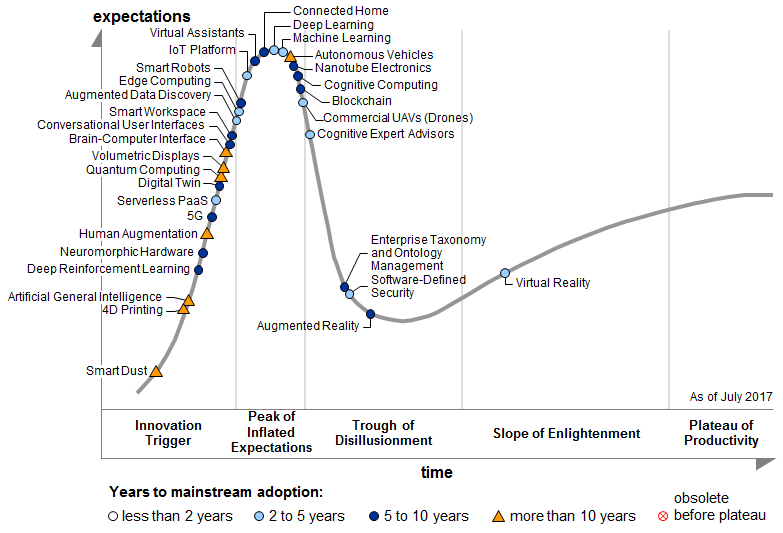
\includegraphics[scale=0.5]{hypecycle2017.png}
\caption[Hype Cycle 2017]{Le tecnologie si muovono lungo l'hype cycle secondo
tempi che possono essere lunghi o brevi (aggiornato al 2017)}
\label{fig:hypecycle2017}
\end{figure}

\subparagraph*{Gartner priority matrix} Identifica le varie tecnologie e ci
associa il livello di impatto che la tecnologia può avere sulle persone.

\section{Significato di un brand}
\begin{definition}[Brand]
Con il termine \textit{brand} si riferisce solitamente al marchio aziendale,
ma, in termini di marketing, fa riferimento ad un contesto più ampio, come al
logo aziendale, alla sua immagine (cui fa parte ad esempio il colore),
l'insieme di valori e a tutti gli aspetti connessi a quello che per noi
rappresenta un determinato marchio. 
\end{definition}

\paragraph*{Terminologia} Un brand presenta i seguenti punti caratteristici:
\begin{itemize}
 \item \textbf{Brand image}: tutto ciò che è connesso al brand tramite
 l'immagine. Rientrano in questa categoria logo, font, nome, colori, \dots{}
 \item \textbf{Brand identity}: ogni brand ha una determinata identità che si
 crea volontariamente o che gli viene associata spontaneamente (a volte anche
 inconsciamente) dagli utenti.
 Spostare la brand identity è difficilissimo, richiede molte risorse e
 investimenti.
 Per questo la reputazione è sempre da tenere sott'occhio, soprattutto oggi
 perché con la diffusione di internet e dei social network è facile diffonderne
 un'opinione negativa.
 Precedentemente al Web 2.0 le aziende erano in una posizione di forza: le
 uniche possibilità per un utente che riscontrava delle problematiche con un
 prodotto o un servizio erano rivolgersi al customer care (e spesso veniva
 di fatto ignorato). Ora è possibile far emergere i problemi di un prodotto su
 social/blog/siti web e la forza di queste lamentele è che gli utenti tendono a
 credere di più a qualcosa che viene da qualcuno simile a loro, piuttosto che
 dall'azienda o dalla pubblicità.
 \item \textbf{Brand reputation}: è la reputazione che un brand ha agli occhi
 degli utenti. Se la reputazione tempo fa era di tipo \textit{broadcast} ovvero
 andava da un punto (l'azienda con la pubblicità) a tutti, oggi è
 ``distribuita'': viene discussa tra la gente e dipende da cosa gli utenti
 dicono di un prodotto.
 \item \textbf{Brand awareness}: quanto è conosciuto un brand, la
 consapevolezza che ciascuno di noi ha di un determinato marchio.
 È uno degli asset più importanti che possono avere le aziende storiche e ben
 strutturate.
 Ci sono vari test per verificare la brand awareness. Uno dei più importanti è,
 tramite delle interviste, chiedere a delle persone di fare una lista di
 aziende che operano in un determinato campo. Le prime aziende saranno quelle
 che più sono impresse nella sua mente, le ultime invece chiederanno
 all'intervistato uno sforzo per essere ricordate. Un altro test è chiedere a
 delle persone di associare un nome ad un certo marchio.
 Le aziende serie lavorano con le \textit{personae}\footnote{Termine inglese 
 per indicare la ``immagine pubblica''}, ovvero con quelle persone di 
 riferimento per  il prodotto di vendita, cercandone determinati valori e 
 caratteristiche.
 Più si identificano le caratteristiche più facile è per determinate persone
 sposare quelle caratteristiche.
 \item \textbf{Brand value}
\end{itemize}
